\documentclass[11pt]{article}  
\usepackage[margin=1in]{geometry}
\parindent=0in
\parskip=8pt
\usepackage{fancyhdr,amssymb,amsmath, graphicx, listings,float,subfig,enumerate,epstopdf,color,multirow,setspace,bm,textcomp}
\usepackage[usenames,dvipsnames]{xcolor}
\usepackage{hyperref}
\usepackage{graphicx}
\usepackage{tikz}
\graphicspath{{./Images}}

\pagestyle{fancy}


\begin{document} 

\lhead{Assignment \# 1}
\chead{Robert Denim Horton}
\rhead{\today}

\begin{center}\begin{Large}
CS 4720/5720 Design and Analysis of Algorithms
Homework \#1
Student: (Robert Denim Horton)
\end{Large}
\end{center}

\section*{Answers to homework problems:}

\textcolor{gray}{
% Chapter 2 : Question 1
\begin{enumerate}
	\item \quad \\
	% Question 1 : Part A
	\begin{enumerate}[(a)]
		\item  Given the formal definition of a pivotal node, a node can be defined as such when the node of interest exists along the \textcolor{red}{only} shortest possible path in a given pair of nodes.  For example, given a graph with the set of nodes $S_0$ with defined nodes $\{A, \ B, \ C, \ D, E\}$.  The graph could be represented as;\\
		\begin{center}
			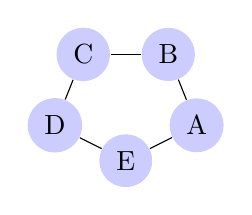
\begin{tikzpicture}[scale=0.9, auto=center, every node/.style={circle,fill=blue!20}] 
				\node(A) at (1, -0.5) {A}; 
				\node(B) at (0.6, 0.5) {B};
				\node(C) at (-0.6, 0.5) {C}; 
				\node(D) at (-1,-0.5) {D}; 
				\node(E) at (0,-1) {E}; 
				\draw(A) -- (B);
				\draw(B) -- (C);
				\draw(C) -- (D);
				\draw(D) -- (E);
				\draw(E) -- (A);
		\end{tikzpicture}
	\end{center}
As we can see in this diagram all the nodes are pivotal nodes.   Starting with pivotal node $A$, its only pivotal node pair is $E$ and $B$, for node $B$ its only pivotal node pair is $C$ and $A$, for node $C$ its only pivotal node pair is $B$ and $D$, for node $D$ its only pivotal node pair is $C$ and $E$, and lastly for node $E$its only pivotal node pair is $D$ and $A$.  Here we can see that every node that exists has at least one pair of nodes that also exists in the graph.\\
% Question 1 : Part B
	\item For a pivotal node to be pivotal to two different pairs of nodes, we can define such a node to be a node that is along the shortest path for two different pairs of nodes. With the same set, $S_0$, from part (a) we can construct a graph as so, 
	\begin{center}
		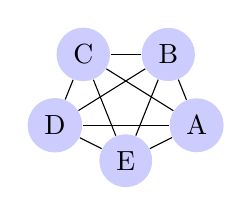
\begin{tikzpicture}[scale=0.9, auto=center, every node/.style={circle,fill=blue!20}] 
			\node(A) at (1, -0.5) {A}; 
			\node(B) at (0.6, 0.5) {B};
			\node(C) at (-0.6, 0.5) {C}; 
			\node(D) at (-1,-0.5) {D}; 
			\node(E) at (0,-1) {E}; 
			\draw(A) -- (B);
			\draw(A) -- (C);
			\draw(B) -- (C);
			\draw(B) -- (D);
			\draw(C) -- (D);
			\draw(C) -- (E);
			\draw(D) -- (E);
			\draw(D) -- (A);
			\draw(E) -- (A);
			\draw(E) -- (B);
		\end{tikzpicture}.
	\end{center}
We can see that for every node in the graph, it has at least two different pairs of nodes that must traverse through this node to get to one another along the shortest path.  Pivotal node $A$ has it's first pivotal nodes as $E$ and $B$ and second pair of pivotal nodes $C$ and $D$,  node $B$ has it's first pair of nodes $C$ and $A$ and second pair of nodes $E$ and $D$, pivotal node $C$ has it's first set of nodes $E$ and $A$ and it's second set of nodes $B$ and $D$, pivotal node $D$ has it's first set of nodes $B$ and $A$ and second pair of nodes $C$ and $E$, pivotal node $D$ has it's first pair of nodes $B$ and $A$ and it's second set of nodes $E$ and $C$, and lastly pivotal node $E$ has it's first pair of nodes $C$ and $B$ and it's second set of nodes $A$ and $D$.\\
% Question 1 : Part C
	\item  For a graph comprised of atleast 4 nodes where a single node is pivotla for any pair of nodes that comprise a pivotal pair.  So with a different set, $S_1$, of nodes \{$A$, $B$, $C$, $D$, $X$\} we can use a graph to represnt a graph where node $X$ is the node of intrest, \\  
	\begin{center}
		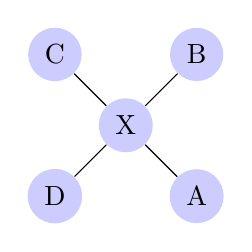
\begin{tikzpicture}[scale=0.9, auto=center, every node/.style={circle,fill=blue!20}] 
			\node(A) at (1, -1) {A}; 
			\node(B) at (1, 1) {B};
			\node(C) at (-1, 1) {C}; 
			\node(D) at (-1,-1) {D}; 
			\node(X) at (0,0) {X}; 
			\draw(A) -- (X);
			\draw(B) -- (X);
			\draw(C) -- (X);
			\draw(D) -- (X);
		\end{tikzpicture}.
	\end{center}
Here we that node $X$ has a pivotla pair with every node that is not $X$ in the graph.  So node $X$ has pivotal pairs $A$ and $C$, pivotal pair $B$ and $D$, pivotal pair $A$ and $B$, pivotal pair $C$ and $B$, pivotal pair $D$ and $A$, and pivotal pair $C$ and $D$. So six possible pairs in total.\\
	\end{enumerate}
\end{enumerate}
}
% Chapter 2 : Question 2
\textcolor{gray}{
\begin{enumerate}
\setcounter{enumi}{1}
	\item \quad \\
	\begin{enumerate}[(a)]
		\item With the formal definetion of a special type of node called a \textit{gatekeeper node}, we can identify gatekeeper node(s) as a node that must be connected by two other nodes that have no other possbile paths or connections between the two connected nodes and are limited to traversing through the gatkeeper node to get to one another  Given a set of nodes, $S_2$, comprised of nodes \{$A$, $B$, $C$, $D$, $E$, $F$\}, we can build a graph with a subset of gatekeeper nodes that comprises more than half the set of nodes in $S_1$.
	\begin{center}
		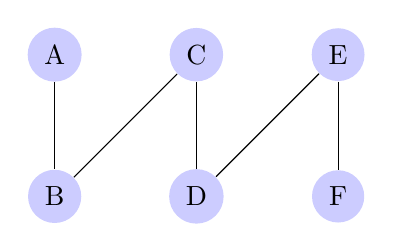
\begin{tikzpicture}[scale=0.9, auto=center, every node/.style={circle,fill=blue!20}] 
			\node(A) at (-2, 1) {A}; 
			\node(B) at (-2, -1) {B};
			\node(C) at (0, 1) {C}; 
			\node(D) at (0, -1) {D}; 
			\node(E) at (2, 1) {E};
			\node(F) at (2, -1) {F};
			\draw(A) -- (B);
			\draw(B) -- (C);
			\draw(C) -- (D);
			\draw(D) -- (E);
			\draw(E) -- (F);
		\end{tikzpicture}.
	\end{center}
As we can see, the subset of nodes \{$B$, $C$, $D$, $E$\} are all gatekeeper nodes tha must be traversed in order for specific pair of nodes to travel to one another via edges.  Further explaining we see that for the of nodes $A$ and $C$ they must travers through node $B$, qualifying node $B$ as a gatekeeper node.  The same can be said for nodes $C$, $D$, and $E$ each be a gatekeeper for their own pair of nodes that they are connected to.  $C$ is a gatekeeper for nodes $B$ and $D$, $D$ is a gatekeeper for nodes $C$ and $E$, and $E$ is a gatekeeper for nodes $D$ and $F$. 
		\item Extendeding the deffinetion of a gatekeeper there are also special kinds of gatekeeper nodes called an \textit{local gatekeeper node}.  These types typed of nodes are also connected by a pair of nodes but does not necessarily be traversed to get from one of node pairs to the other.  Given the set, $S_3$, of nodes \{$A$, $B$, $C$, $D$\} we can build a graph that consists of \textbf{only local gatekeeper nodes}.  The graph would look like;
 	\begin{center}
		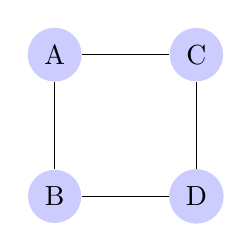
\begin{tikzpicture}[scale=0.9, auto=center, every node/.style={circle,fill=blue!20}] 
			\node(A) at (-2, 1) {A}; 
			\node(B) at (-2, -1) {B};
			\node(C) at (0, 1) {C}; 
			\node(D) at (0, -1) {D}; 
			\draw(A) -- (B);
			\draw(B) -- (D);
			\draw(D) -- (C);
			\draw(C) -- (A);
		\end{tikzpicture}.
	\end{center}
As can be seen from this graph, we notice that every pair of nodes that aren't directly connected have multiple paths or traversal to get to on another.  For example, nodes $A$ and $D$ have two paths of traversal to get to one another.  They can traverse through the first local gatekeeper, $B$, or they can traverse to each other through the second local gatekeeper $C$.  The logic can be tested on any pairs of nodes in this graph, that are not directly connected, and the conclusion will be that for every one of these pairs of nodes, there are two local gatekeeper nodes.  After stepping through the logic for every pair of nodes we will find that every node in this graph is a local gatekeeper node.
	\end{enumerate}
\end{enumerate}
}

% Chapter 2 : Question 3
\textcolor{gray}{
\begin{enumerate}
\setcounter{enumi}{2}
	\item \quad \\
	\begin{enumerate}[(a)]
		\item To first construct such a graph lets first formally define \textit{diameter} and \textit{average distance} of a graph.  The \textit{\textbf{diameter}} of a graph can be found by simply finding the longest shortest path that connects two nodes in the graph  This is to say, find the two nodes on the graph that are furthest apart from and other two nodes on the graph and find the longest path in between these two nodes.  To find the \textit{\textbf{average distance}} there are several different ways this can be done and usually a \textit{Breath first search} implementation can make things easier when calculating the avg. distance.  However, for a smaller and simpler looking graph, we can look through each pair of nodes that has a connection (or series of connections) and then add up all the edges that connect each combination of possible pairs of nodes along the shortest path.  We then divide this sum using the number of nodes, $n$, that exsist on the graph along with what is called the \textit{Weilder index}  The Weiner index is a number that corresponds to the number of connected nodes in the graph.  With this number we then divide the sum of all the distances and divide them by this weiner index.  With the provided knowledge of how to find the \textit{diameter} and \textit{average distance} we can then start to build a graph where the diameter is at least three time larger than the average distance.\\\\
To give an example we can start with a set, $S_4$, of nodes \{$A$, $B$, $C$, $D$\} we construct the first part of the graph where the nodes $A$, $B$, and $C$ are each closely connected to its next corresponding node with a single node. An illustration is provided below of our first part of the graph.
   	\begin{center}
		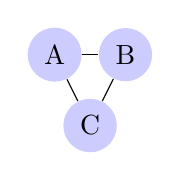
\begin{tikzpicture}[scale=0.9, auto=center, every node/.style={circle,fill=blue!20}] 
			\node(A) at (-0.5, 1) {A}; 
			\node(B) at (0.5, 1) {B};
			\node(C) at (0, 0) {C}; 
			\draw(A) -- (B);
			\draw(B) -- (C);
			\draw(C) -- (A);
		\end{tikzpicture}.
	\end{center}
We can then observe that the average distance is one within the first part of the graph.  We can prove this through our formal definition by going through and adding up all the shortest distances for every possible combination of pairs of nodes that are connected, with out revisting the same nodes in a traversal. So we get, 
	\begin{center}
		\begin{tabular}{||c | c||} 
	 		\hline
	 		Pair of Nodes & Distance  \\ [0.5ex] 
			\hline
			 ($A$, $B$) & 1  \\ 
			 \hline
			 ($A$, $C$) & 1  \\ 
			 \hline
			 ($C$, $B$) & 1  \\ 
			 \hline\hline
			 SUM &  3\\
			\hline
		\end{tabular}
	\end{center}
We can then take this sum and divide it by the number of connected nodes that build of this first part of the graph, 3.  After dividing the sum by the amount number of connected nodes we get 1.   Continuing from here we add in our last node, $F$ , with a single edge connected to node $C$ yeilding our full graph below, 
   	\begin{center}
		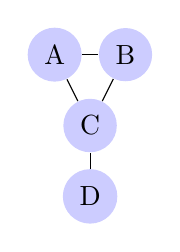
\begin{tikzpicture}[scale=0.9, auto=center, every node/.style={circle,fill=blue!20}] 
			\node(A) at (-0.5, 1) {A}; 
			\node(B) at (0.5, 1) {B};
			\node(C) at (0, 0) {C}; 
			\node(D) at (0, -1) {D};
			\draw(A) -- (B);
			\draw(B) -- (C);
			\draw(C) -- (A);
			\draw(C) -- (D);
		\end{tikzpicture}.
	\end{center}
By adding this node to our already constructed graph, we make several more connections between the already existing nodes.  
	\begin{center}
		\begin{tabular}{||c | c||} 
	 		\hline
	 		Pair of Nodes & Distance  \\ [0.5ex] 
			\hline
			 ($A$, $B$) & 1  \\ 
			 \hline
			 ($A$, $C$) & 1  \\ 
			 \hline
			 ($C$, $B$) & 1  \\ 
			 \hline
			 ($C$, $D$) & 1  \\ 
			 \hline
			 ($A$, $D$) & 2  \\ 
			 \hline
			 ($B$, $D$) & 2  \\ 
			 \hline\hline
			 SUM &  8\\
			\hline
		\end{tabular}
	\end{center}
We can now see that our sum of distances is 8 which we can now divide by the total number of exsisting connected nodes in this completed graph (6).  So, our average distance is 8/6.  Now that we have constructed our graph we can simply find the diameter of the graph by finding the longest path to traverse this graph.  In this case it would be from node  $B$ to node $A$, then from node $A$ to node $C$, and finally from node $C$ to node $D$.  Counting up all the edges traversed from node $B$ to node $D$ we find the diameter is 3.  Comparing our avg. distance to the diameter of the graph we find that the diameter is at least three times the avg. distance.
		\item To expand on our example of a graph where the diameter is three times the size of the avg distance we can call the first part of the graph that we constructed as the \textcolor{red}{\textit{large component}}. We will also denote the number of nodes that exists in this part of the graph as $c$.  So for our first example the number of nodes in this \textcolor{red}{larger component} was three.  The second part of the graph we constructed contained what we will refer to as the outer nodes that are connected to the \textcolor{red}{larger component} but is not directly related to amount of nodes, $c$, in this part of the graph.  Continuing with our previous example we observed that with our . . . . \textcolor{gray}{Describe how you could extend your construction to produce graphs in which the diameter exceeds the average distance by as large a factor as you’d like. (That is, for every number c, can you produce a graph in which the diameter is more than c times as large as the average distance?)}\\
	\end{enumerate}
\end{enumerate}
}
\end{document}
